\chapter{Results}\label{section:results}

    Here we present the results from our two different experiments.

    We compare the results of our code-prose experiment to the original study~\cite{floyd_decoding_2017} and the replication study~\cite{fucci_replication_2019}, and investigate the results from our naturalistic device use experiment to see if results generalize to other types of device activity.

    \todo[inline]{Update with final values}

    \section{Code vs prose task}

        Our top-performing classifier, using LORO cross-validation, yields a median BAC score of $0.749$  for window-level classification and $0.9$ for epoch-level classification (seen in Table~\ref{table:bac-selective}).

        The top-performing classifier computes the covariance matrices, and then uses using Riemannian geometry, Common Spatial Pattern, and TangentSpace. With logistic regression for the final step.

        We do window-level classification by training on the \SI{5}{\second} windows (as described in Section~\ref{section:transform}).

        We achieve epoch-level classification by training a window-level classifier just as for the \SI{5}{\second} windows, we then make a classification for the entire epoch by taking the mean of the prediction probabilities from the windows in that epoch.

        \todo[inline]{Markus: Vilken modell är det som gäller nu? Och vilka features och clearning och sånt bygger den på? Kanske avsluta kapitel 3 med att tydligt presentera vad som används i experimenten?}
        
        \begin{comment}
            The following is the performance statistics for our model trained on \SI{5}{\second} windows. It is trained on all subjects except one, which is used in testing:

            \begin{verbatim}
            INFO: {
                'precision': 0.7473868367437329, 
                'recall': 0.696405129166862, 
                'fbeta': 0.6703482474923927, 
                'support': array([308, 277]), 
                'bac': 0.696405129166862, 
                'confusion_matrix': array([[141, 167], [ 18, 259]])
            }
            \end{verbatim}

            The following are the performance statistics for our model on the epoch-level.  The same subject selection as the previous statistics is used:

            \begin{verbatim}
            INFO: {
                'precision': 0.8541666666666667, 
                'recall': 0.7666666666666666, 
                'fbeta': 0.7624602332979852, 
                'support': array([15, 17]), 
                'bac': 0.7666666666666666, 
                'confusion_matrix': array([[ 8,  7], [ 0, 17]])
            }
            \end{verbatim}
        \end{comment}

        \begin{table}[h]
            \centering
            \begin{tabular}{lcc}
            \toprule
                \textbf{Subject} & \textbf{Window-level} & \textbf{Epoch-level} \\
            \midrule
            \#0  & 0.608  & 0.603 \\
            \#1  & 0.802  & 0.864 \\
            \#5  & 0.589  & 0.534 \\
            \#6  & 0.701  & 0.767 \\
            \#7  & 0.694  & 0.8   \\
            \#8  & 0.547  & 0.542 \\
            \#9  & 0.484  & 0.5   \\
            \#10 & 0.474  & 0.5   \\
            \midrule
            Median & 0.5985 & 0.573 \\
            \bottomrule
            \end{tabular}
            \caption{The BAC score for each LORO fold/subject. Excluding subjects 3 and 4.}\label{table:bac-all}
        \end{table}


        \begin{table}[h]
            \centering
            \begin{tabular}{lcc}
            \toprule
                \textbf{Subject} & \textbf{Window-level} & \textbf{Epoch-level} \\
            \midrule
            \#0 & 0.673 & 0.727 \\
            \#1 & 0.895 & 0.955 \\
            \#5 & 0.616 & 0.542 \\
            \#6 & 0.864 & 0.908 \\
            \#7 & 0.749 & 0.9   \\
            \midrule
            Median & 0.749 & 0.9 \\
            \bottomrule
            \end{tabular}
            \caption{The BAC score for each LORO fold/subject. Excluding subjects 3, 4, 8, 9, and 10.}\label{table:bac-selective}
        \end{table}

        \begin{table}
            \begin{center}
                \begin{tabular}{lcc}
                  \toprule
                            & Epoch-level (subject \#6) & Window-level (subject \#6) \\
                  \midrule
                  Precision & 85.4\%                    & 74.7\% \\
                  BAC       & 76.7\%                    & 69.6\% \\
                  \bottomrule
                \end{tabular}
                \caption{Performance statistics of our models trained on all subjects with good signal quality, except subject number \#6 which is used for testing.}\label{fig:stats}
            \end{center}
        \end{table}

        %\begin{figure}[h]
        \begin{landscape}
            \begin{figure}
                \centering
                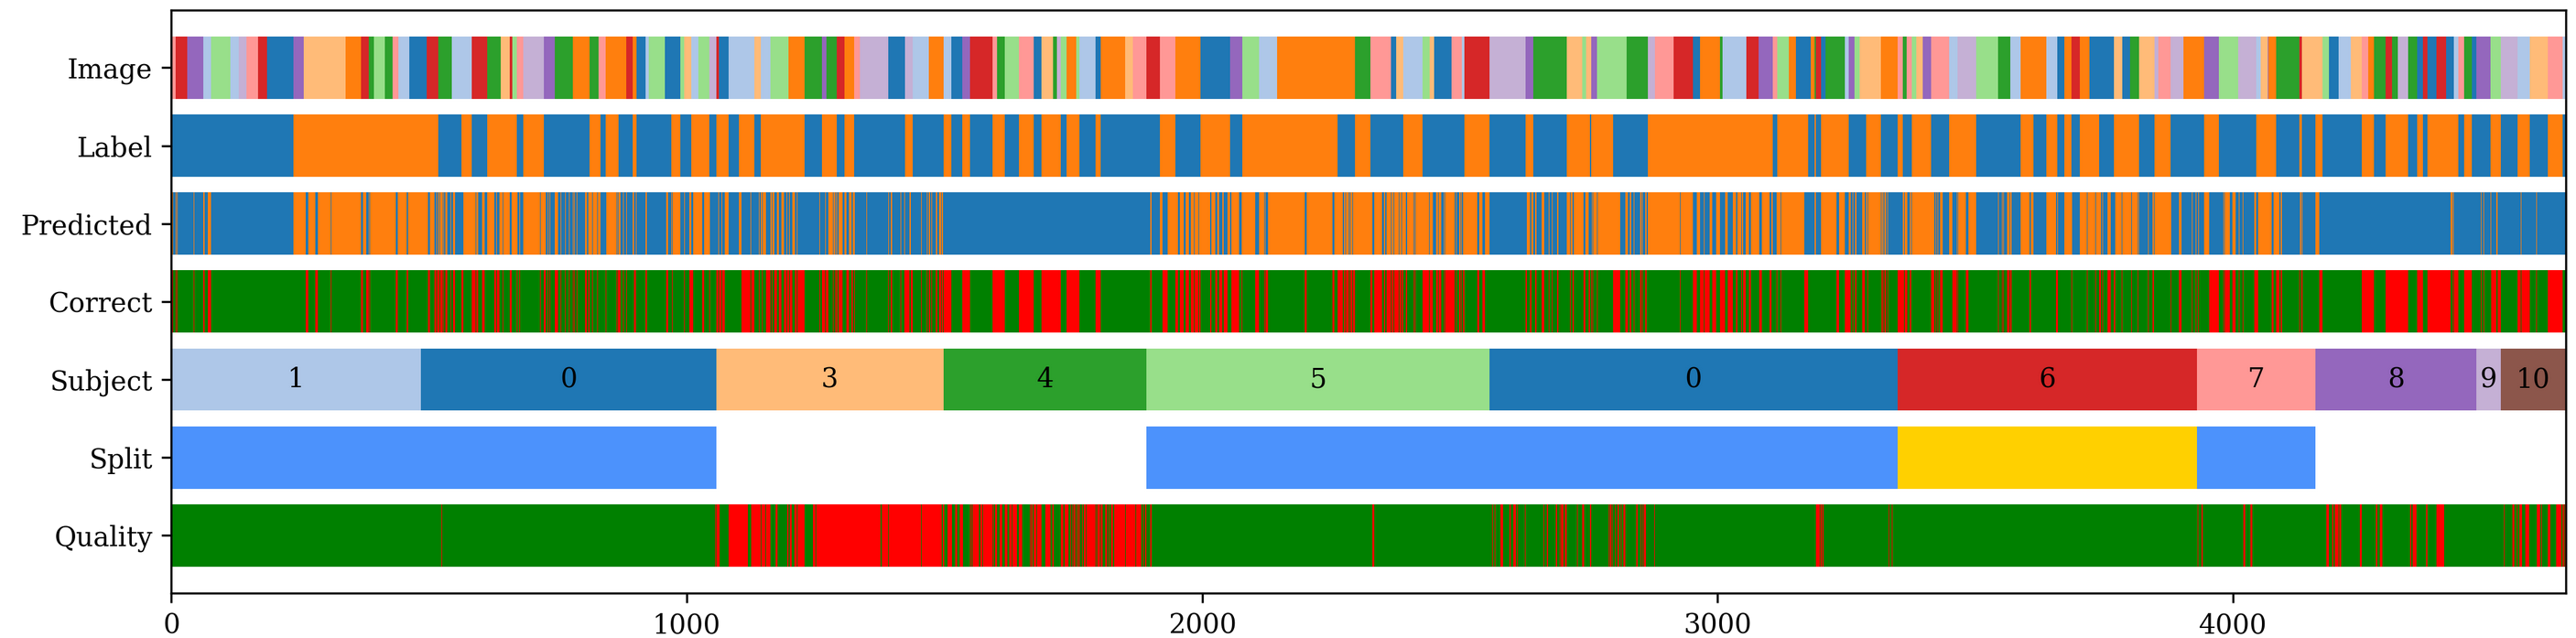
\includegraphics[width=24cm]{img/timebars.png}
                \caption{Visualization of the labeled data. Shows the \emph{image} (stimuli), the \emph{label} for that stimuli, the \emph{predicted} class, whether the prediction is \emph{correct}, the \emph{subject}, the \emph{training} and \emph{testing} split, and a measure of signal \emph{quality}. The x-axis is the window index, sorted by acquisition time.
                \\ 
                \\
                It can be seen that subjects \#3 and \#4 have bad signal quality, and have therefore been excluded from the training set. The last two subjects have also been excluded from training due to issues during data collection. It can also be seen that for subject \#1 the stimuli images were not shuffled.}\label{fig:timebars}
            \end{figure}
        \end{landscape}
        %\end{figure}

        \begin{comment}
            \begin{figure}[h]
            \centering
            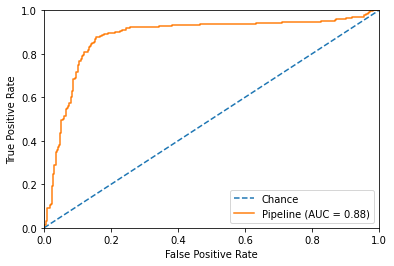
\includegraphics[width=12cm]{img/roccurve.png}
            \caption{Receiver operating characteristic (ROC) curve for subject \#6.}\label{fig:roc}
            \end{figure}
            \todo[inline]{Update with higher-res image}
        \end{comment}

        Compared to previous studies, we achieve a moderate improvement over the EEG-only classifier trained in Fucci et al., and achieve a similar performance to the fMRI study by Floyd et al. (seen in Table~\ref{table:compare-results}).

        \begin{table}
            \begin{center}
                \begin{tabular}{lccc}
                    \toprule
                    & \textbf{This study} & \textbf{Fucci et al.} & \textbf{Floyd et al.} \\
                    \midrule
                    Overall & 0.75 & 0.66 & 0.79 \\
                    Code & x & x & x \\
                    Prose & x & x & x \\
                    \bottomrule
                \end{tabular}
                \caption{Result comparison between the previous studies and this study. Best BAC results are reported. For Fucci et al.\ we chose the best EEG-only score.}\label{table:compare-results}
            \end{center}
        \end{table}

    \section{Naturalistic device activity}

        We collected TODO hours of EEG data during natural device use.

        We use the classes defined in Section~\ref{section:collect-usage}.

        We train classifiers for the label pairs:

        \begin{itemize}
                \item Editing Code / Editing Prose
                \item Editing Code / Twitter
                \item Twitter / YouTube
        \end{itemize}

        The class distribution is as follows: TODO

        Our classifier performance is: TODO

